\section{Results}

\subsection{MRI in self-gravitating polytropic disks with uniform
  resistivity}  
We first calculate the MRI as a function of $Q$ in a polytropic disk
with uniform resistivity ($A=1$). We consider $Q\in[0.2,4]$,
corresponding to stronly self-gravitating to non-self-gravitating
disks, for mid-plane Elsasser numbers $\Lambda_0\in[0.3,5]$. 
We fix $k_x=0.1$ and $\beta=100$. The numerical resolution is
$N_z=256$. 

Fig. \ref{compare_growth_poly_uniresis} plots the MRI growth rates as
a function of $Q$ and $\Lambda_0$. As expected growth rates generally
decrease with $\Lambda_0$. In the limit of ideal MHD, $\Lambda_0>1$,
there is negligible dependence on $Q$. In the resistive limit,
$\Lambda_0<1$, growth rates decrease noticeably for $Q<1$. This shows
show that self-gravity can still affect the MRI even  
though density and potential perturbations are expected to be
negligible because $k_x\ll1$ (i.e. the linear response is
non-self-gravitating).    
 
\begin{figure}
  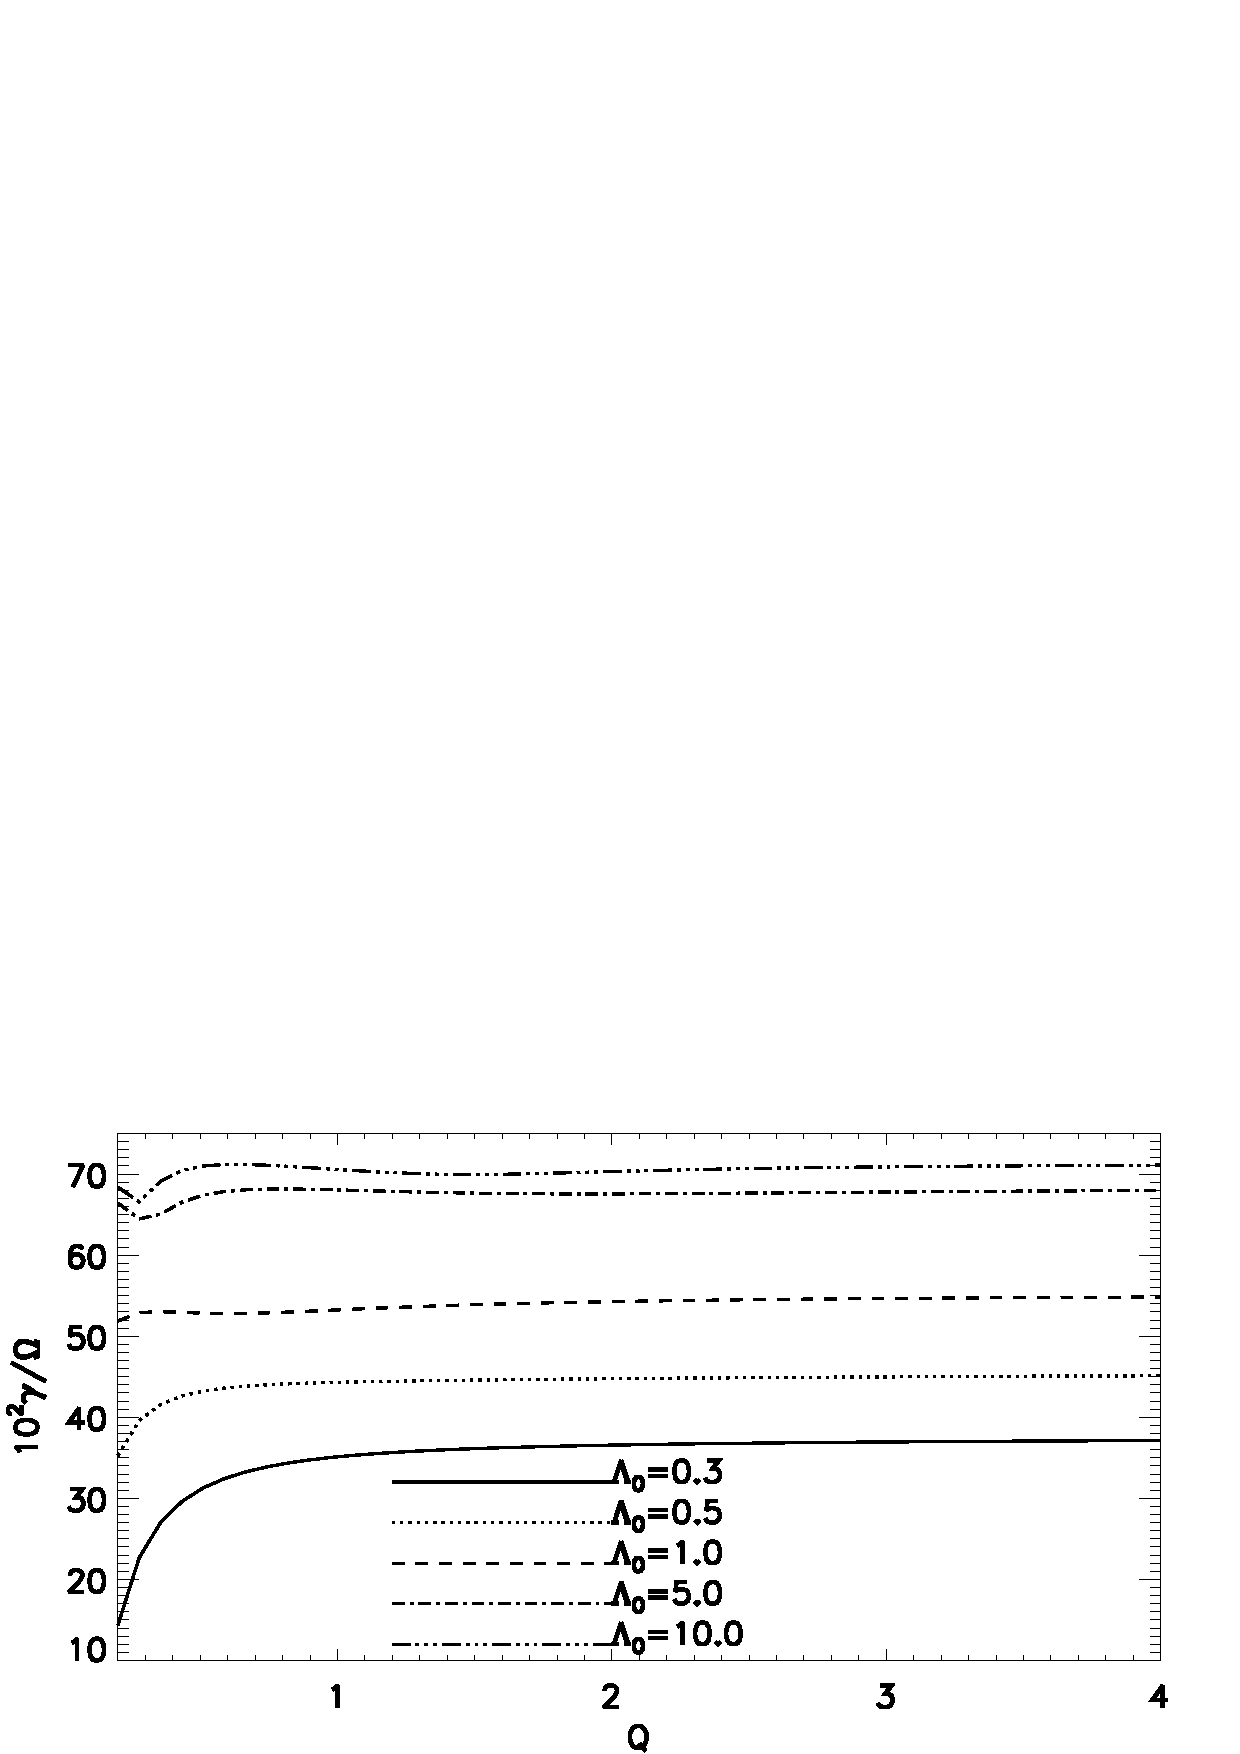
\includegraphics[width=\linewidth]{figures/compare_growth_poly_uniresis}
  \caption{MRI growth rates as a function of $Q$ for mid-planet
    Elsasser numbers $\Lambda_0=0.3$ (solid), $0.5$ (dotted), $1.0$
    (dashed) and $5.0$ (dash-dot).  
    \label{compare_growth_poly_uniresis}}
\end{figure}

% (We find the weak variations in
%$\gamma$ for small $Q$ is associated with a change in the number of
%nodes in the magnetic field perturbation.)
%because $f$ is of order unity for the
%range of $Q$ considered so $\lambda_\mathrm{ideal}$ remain less than
%  unity.
%However, in the resistive limit, the dependence of
%  $\lambda_\mathrm{resis}$ on $f$ (and hence $Q$) is amplified by
%  $\Lambda_0 < 1$.

\cite{sano99} found that for instability to occur the linear mode
dimensional wavelength $\lambda$ should fit inside the disk. That is,   
\begin{align}\label{sano_crit}
  \frac{\lambda}{2H} \equiv
  \mathrm{max}\left(\lambda_\mathrm{ideal},\lambda_\mathrm{resis}\right)\lesssim
  1, 
\end{align}
where the non-dimensional wavelengths are given by 
\begin{align}\label{lambda_ideal}
  \lambda_\mathrm{ideal} = \frac{4\pi}{\sqrt{15}} f v_A =
  \frac{4\pi f}{\sqrt{15\beta\rho}}
\end{align}
in the limit of ideal MHD, and 
\begin{align}\label{lambda_resis}
  \lambda_\mathrm{resis} = \frac{2\pi}{\sqrt{3}}\frac{\eta}{v_A f} =
  \frac{2\pi f}{\Lambda_0}\sqrt{\frac{\rho}{3\beta}} 
\end{align}
%factor pi comes form converting vertical wavenumber to
%wavelength. linear theory works with wavenumber, physical
%interpretation in terms of wavelengths
in the limit of high resistivity. 
%For $\Lambda_0\gtrsim 1$, we find
%the condition $\lambda < 2H$ is well-satisifed throughout most of the
%disk regardless of $Q$.     
For polytropic disks the normalized density $\rho$ is weakly dependent
on $Q$ (Fig. \ref{eqm_den}) so self-gravity only affects the
MRI through the factor $f$, which increases with decreasing $Q$ (see
Fig. \ref{plot_fq} in Appendix \ref{appen1}). This suggests that
sufficiently strong self-gravity can stabilize the MRI by making
$\lambda > 2H$. 
 
%Physically, the
%disk becomes thinner with increasing self-gravity, and the MRI will be
%surpressed when the disk is too thin to accommodate unstable modes. 
%MRI requires
%$\lambda\lesssim 1$, so that the unstable wavelength fits within the
%disk column. As shown in Appendix \ref{appen1}, $f$ increases with the
%strength of self-gravity. This is expected to increase $\lambda$ and
%weaken the MRI.  

However, $f$ does not vary much for the range of $Q$ considered here. 
In the ideal limit, we find $\lambda < 2H$ throughout most of the disk
for all values of $Q$, so that self-gravity does not affect growth
rates significantly. Weak variations in $\gamma$ were found to be
associated with changes in the 





\begin{figure}
  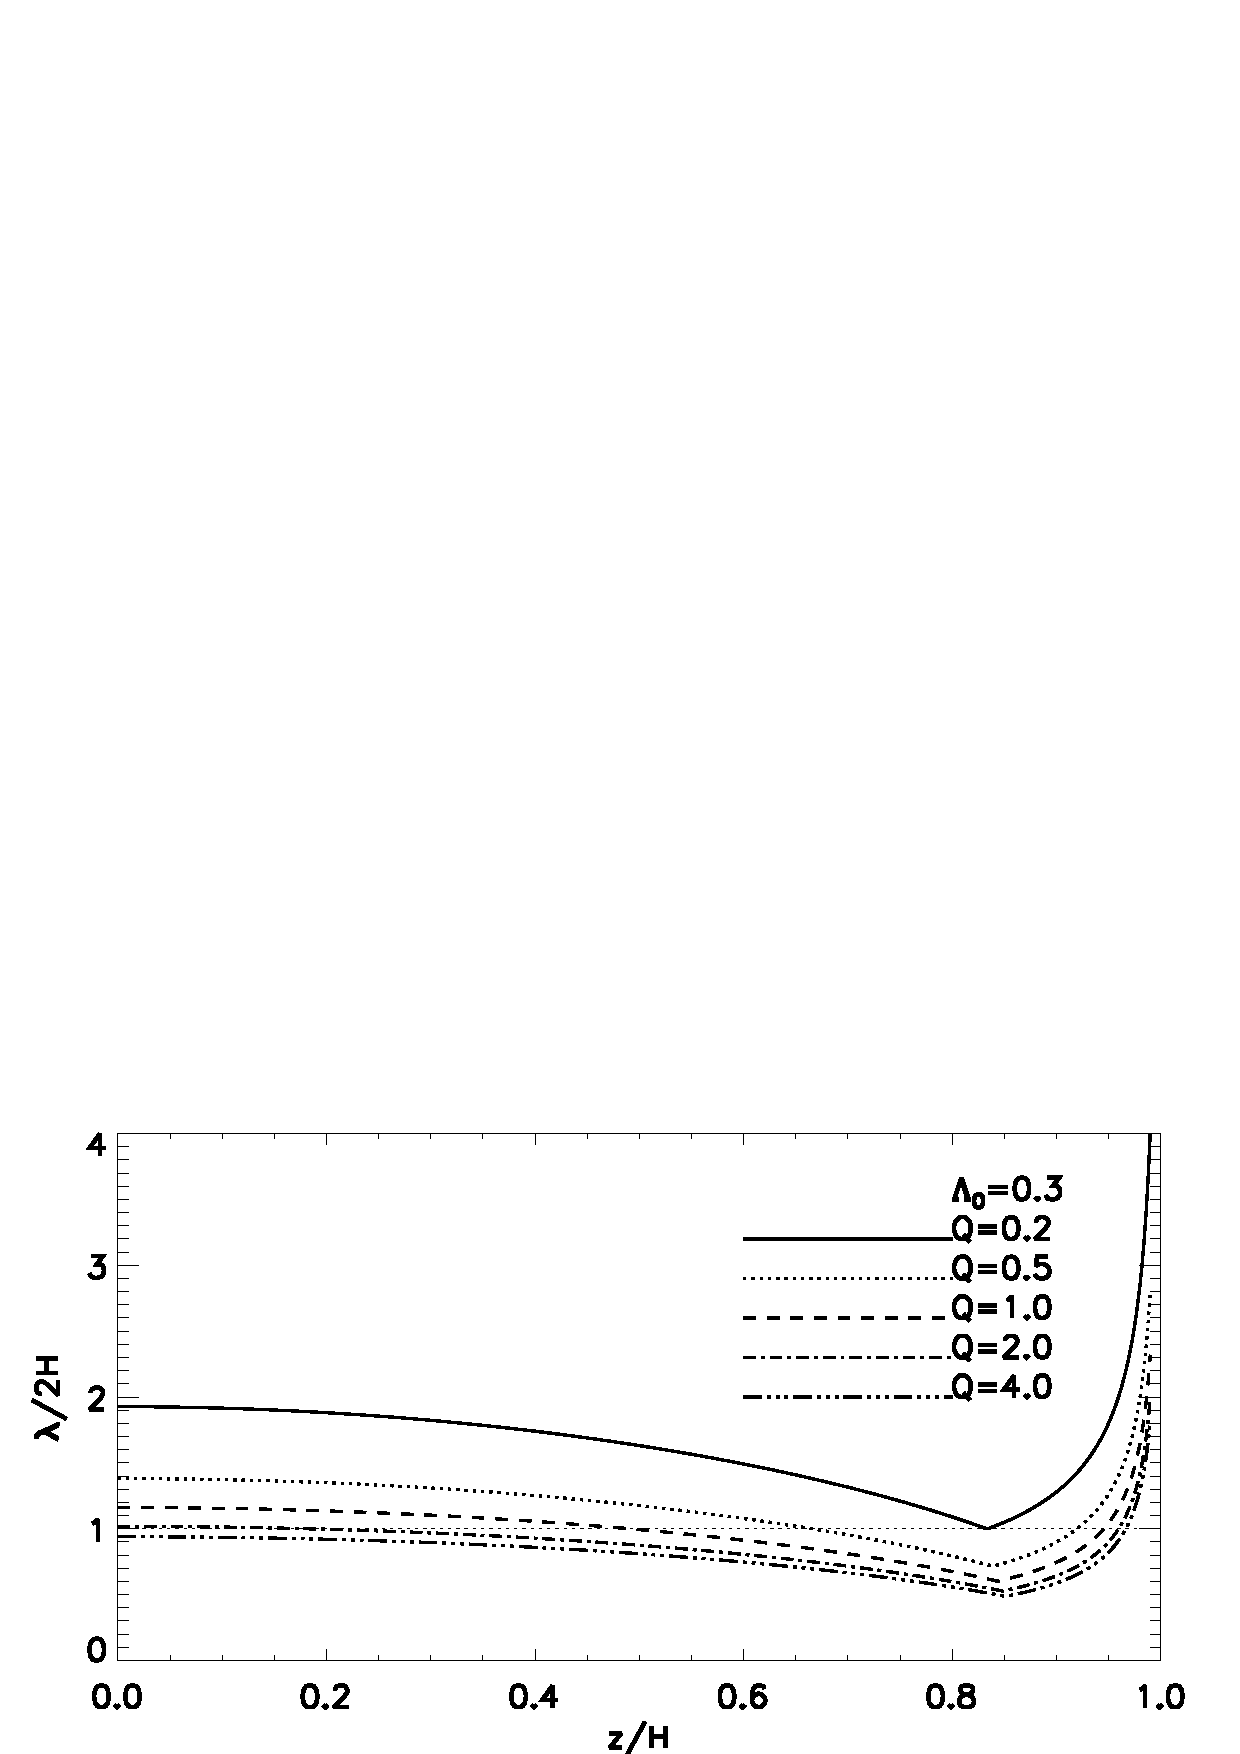
\includegraphics[width=\linewidth]{figures/lambda_poly_uniresis}
  \caption{Wavelength of the most unstable resistive MRI modes as given by
    Eq. \ref{sano_crit}---\ref{lambda_resis}, normalized by the 
    disk thickness, as a function of height for a range of Toomre $Q$
    values.  
    \label{lambda_poly_resis}}
\end{figure}


\subsection{Resistive MRI in massive polytropic disks with layered
  resistivity} 


\subsection{GI in magnetized isothermal disks with uniform
  resistivity} 


\subsection{GI in magnetized isothermal disks with layered
  resistivity} 
